% Options for packages loaded elsewhere
\PassOptionsToPackage{unicode}{hyperref}
\PassOptionsToPackage{hyphens}{url}
%
\documentclass[
]{article}
\usepackage{amsmath,amssymb}
\usepackage{lmodern}
\usepackage{ifxetex,ifluatex}
\ifnum 0\ifxetex 1\fi\ifluatex 1\fi=0 % if pdftex
  \usepackage[T1]{fontenc}
  \usepackage[utf8]{inputenc}
  \usepackage{textcomp} % provide euro and other symbols
\else % if luatex or xetex
  \usepackage{unicode-math}
  \defaultfontfeatures{Scale=MatchLowercase}
  \defaultfontfeatures[\rmfamily]{Ligatures=TeX,Scale=1}
\fi
% Use upquote if available, for straight quotes in verbatim environments
\IfFileExists{upquote.sty}{\usepackage{upquote}}{}
\IfFileExists{microtype.sty}{% use microtype if available
  \usepackage[]{microtype}
  \UseMicrotypeSet[protrusion]{basicmath} % disable protrusion for tt fonts
}{}
\makeatletter
\@ifundefined{KOMAClassName}{% if non-KOMA class
  \IfFileExists{parskip.sty}{%
    \usepackage{parskip}
  }{% else
    \setlength{\parindent}{0pt}
    \setlength{\parskip}{6pt plus 2pt minus 1pt}}
}{% if KOMA class
  \KOMAoptions{parskip=half}}
\makeatother
\usepackage{xcolor}
\IfFileExists{xurl.sty}{\usepackage{xurl}}{} % add URL line breaks if available
\IfFileExists{bookmark.sty}{\usepackage{bookmark}}{\usepackage{hyperref}}
\hypersetup{
  pdftitle={On the inference of positive and negative species associations and their relation to abundance},
  hidelinks,
  pdfcreator={LaTeX via pandoc}}
\urlstyle{same} % disable monospaced font for URLs
\usepackage[margin=1in]{geometry}
\usepackage{graphicx}
\makeatletter
\def\maxwidth{\ifdim\Gin@nat@width>\linewidth\linewidth\else\Gin@nat@width\fi}
\def\maxheight{\ifdim\Gin@nat@height>\textheight\textheight\else\Gin@nat@height\fi}
\makeatother
% Scale images if necessary, so that they will not overflow the page
% margins by default, and it is still possible to overwrite the defaults
% using explicit options in \includegraphics[width, height, ...]{}
\setkeys{Gin}{width=\maxwidth,height=\maxheight,keepaspectratio}
% Set default figure placement to htbp
\makeatletter
\def\fps@figure{htbp}
\makeatother
\setlength{\emergencystretch}{3em} % prevent overfull lines
\providecommand{\tightlist}{%
  \setlength{\itemsep}{0pt}\setlength{\parskip}{0pt}}
\setcounter{secnumdepth}{-\maxdimen} % remove section numbering
\usepackage{xr}
\externaldocument{RarePlusComMinus_supp}
\usepackage{lineno}
\ifluatex
  \usepackage{selnolig}  % disable illegal ligatures
\fi
\newlength{\cslhangindent}
\setlength{\cslhangindent}{1.5em}
\newlength{\csllabelwidth}
\setlength{\csllabelwidth}{3em}
\newenvironment{CSLReferences}[2] % #1 hanging-ident, #2 entry spacing
 {% don't indent paragraphs
  \setlength{\parindent}{0pt}
  % turn on hanging indent if param 1 is 1
  \ifodd #1 \everypar{\setlength{\hangindent}{\cslhangindent}}\ignorespaces\fi
  % set entry spacing
  \ifnum #2 > 0
  \setlength{\parskip}{#2\baselineskip}
  \fi
 }%
 {}
\usepackage{calc}
\newcommand{\CSLBlock}[1]{#1\hfill\break}
\newcommand{\CSLLeftMargin}[1]{\parbox[t]{\csllabelwidth}{#1}}
\newcommand{\CSLRightInline}[1]{\parbox[t]{\linewidth - \csllabelwidth}{#1}\break}
\newcommand{\CSLIndent}[1]{\hspace{\cslhangindent}#1}

\title{On the inference of positive and negative species associations
and their relation to abundance}
\author{}
\date{\vspace{-2.5em}}

\begin{document}
\maketitle

\linenumbers

\begin{quote}
\hypertarget{abstract}{%
\subsubsection{Abstract}\label{abstract}}
\end{quote}

\begin{quote}
The prevalence of rare species in ecosystems begs the question of how
they persist. In a recent paper, Calatayuda et al.~(CEA) provided a new
hypothesis that rare species, in contrast to common species, share
unique microhabitats and/or preferentially engage in mutualistic
interactions. CEA support this hypotheses by reconstructing association
networks from spatially replicated abundance data finding that rare
species are over-representing in positive association networks while
common species are over-representing in negative association networks.
However, the use of abundance and co-occurrence data to infer true
species associations is difficult and often inaccurate. Here, I show
that the finding of rare species being more represented in positive
association networks can be explained by statistical artifacts in the
inference of species associations from abundance data. I caution against
the inference of ecological association networks from abundance data
alone. \newline \newline
\end{quote}

Why do rare species persist in ecosystems? Rare species seem to be at a
disadvantage by pure probabilistic odds (McGill \emph{et al.}, 2005) and
perhaps also from poorly adapted species-environment and species-species
interactions (Hutchinson, 1961), though negative density-dependence may
help buoy rare species (Leigh Jr \emph{et al.}, 2004; Yenni \emph{et
al.}, 2012). The question of rarity and persistence thus remains
unresolved. In a recent paper, Calatayud \emph{et al.} (2019) (CEA) have
contributed toward helping resolve this question. They compiled an
impressive collection of datasets, across many taxa and environments,
capturing spatially replicated species abundance measures. With these
data they inferred species-species association networks. Such
association networks are hypothesized to reflect both potential
species-species interactions and/or shared environmental preferences,
though there is debate about their accuracy and interpretation (Sander
\emph{et al.}, 2017; Barner \emph{et al.}, 2018; Freilich \emph{et al.},
2018; Carr \emph{et al.}, 2019; Rajala \emph{et al.}, 2019; Blanchet
\emph{et al.}, 2020). CEA found that rare species were statistically
over-represented in positive-positive species association networks,
while common species were statistically over-represented in
negative-negative species association networks (Calatayud \emph{et al.},
2019). CEA interpreted this finding as possible evidence that the
persistence of rare species may be aided by positive species
interactions, such as mutualism or facilitation, or by shared use of
similar microhabitats. However, this result could be compromised by the
unreliability of inferring species associations from abundance data
alone. Here, I show that the correlation between abundance and
association type (positive or negative) as reported by CEA can be
explained by statistical artifacts. These artifacts arise because of
spatial clustering in intra-specific abundances. It would therefore not
be supported to assign biological interpretations to correlations
between association types and abundances until more data can be brought
to bear on the subject.

When association networks are inferred from spatially replicated
abundance data, species-species co-occurrences are quantified by a
metric (e.g., CEA use Schoener similarity (Schoener, 1968)) and then a
null model is used to assess whether these co-occurrence metrics deviate
substantially enough from null expectations to suggest a non-random
association, either in the positive or negative direction. However,
seemingly non-random patterns in abundance can arise from many
processes, including neutrality, that are not driven by species
interactions or associations. As such, deviations of abundance patterns
from null models might not, by itself, indicate true associations or
interactions. One critical, and widely observed, property of species
abundances is that they are not evenly distributed across species nor
across space within a given species (often referred to as spatial
clustering) (McGill \& Collins, 2003; Engen \emph{et al.}, 2008; Zillio
\& He, 2010; Harte, 2011; Connolly \emph{et al.}, 2017). Both ubiquitous
patterns can be accounted for by purely probabilistic processes from
neutral birth-death-immigration (Kendall, 1949; Hubbell, 2001) to
mechanistically agnostic statistical-mechanical properties of large
assemblages (Harte, 2011). Importantly, the negative binomial
probability distribution both accurately reflects many empirical
measurements of spatial variation in intra-specific abundances (Harte,
2011; Connolly \emph{et al.}, 2017) and is independently derived by
disparate null or neutral ecological theories (Kendall, 1949; Engen
\emph{et al.}, 2008; Harte, 2011).

Thus, the simple observation of uneven or clustered intra-specific
abundances does by itself indicate the influence of deterministic
species associations. The data compiled by CEA (Calatayud \emph{et al.},
2019) indeed confirm the ubiquity of uneven species abundances both at
an intra-specific level across space (Supplementary Fig. \ref{fig:ssad})
at an inter-specific level (Supplementary Fig. \ref{fig:sadShape}). For
consistency, I will refer to the spatial distribution of intra-specific
abundances as the spatial species abundance distribution (SSAD)
following Harte (Harte, 2011) and the inter-specific distribution of
abundances as the species abundance distribution SAD. To reiterate for
clarity, the SSAD is a measure of spatial variability in
\emph{intra}-specific abundances across space and is measured once for
each species; the SAD is a measure of variability in abundance across
species (i.e.~\emph{inter}-specific abundances).

Using simulation, I show that intra-specific spatial clustering of the
SSAD alone is sufficient to reproduce the apparent correlation between
abundance and association type reported by CEA. Spatial clustering is
not, by itself, evidence that rare species positively associate with
each other while common species negatively associate. Therefore, the
observations reported by CEA do not tell us about species associations,
but rather that the null models used do not preserve important aspects
of the SSAD.

In Figure \ref{fig:plusMinus} I first reproduce key results from CEA's
Figure 2(B-C). Then to evaluate whether these results can be produced
simply from spatial clustering alone I simulate purely random data (with
absolutely no association or interaction between species) that match the
unevenness of abundances found in the observed data. These random data
are simulated as follows:

\begin{enumerate}
\def\labelenumi{\arabic{enumi})}
\tightlist
\item
  The number of species \(S\), number of sites \(M\), and shape of the
  best fitting SAD are sampled (with replacement) from the observed data
\item
  \(S\) species abundances \(x_i \ldots x_S\) are sampled from the SAD
\item
  For each species \(i\) with abundance \(x_i\), within-species counts
  are distributed across the \(M\) sites according to an SSAD that is
  either negative binomial (in the case of spatial clustering) or
  Poisson (in the case of spatial randomness)
\item
  The resulting simulated site by species matrix is fed through the same
  analytically pipeline (described in CEA) as the observed data to infer
  positive and negative associations.
\end{enumerate}

All analyses are carried out in R (R Core Team, 2018) and can be fully
reproduced by installing the R package
(\url{https://github.com/ajrominger/RarePlusComMinus}) accompanying this
paper, as detailed in the supplement.

\begin{figure}

{\centering 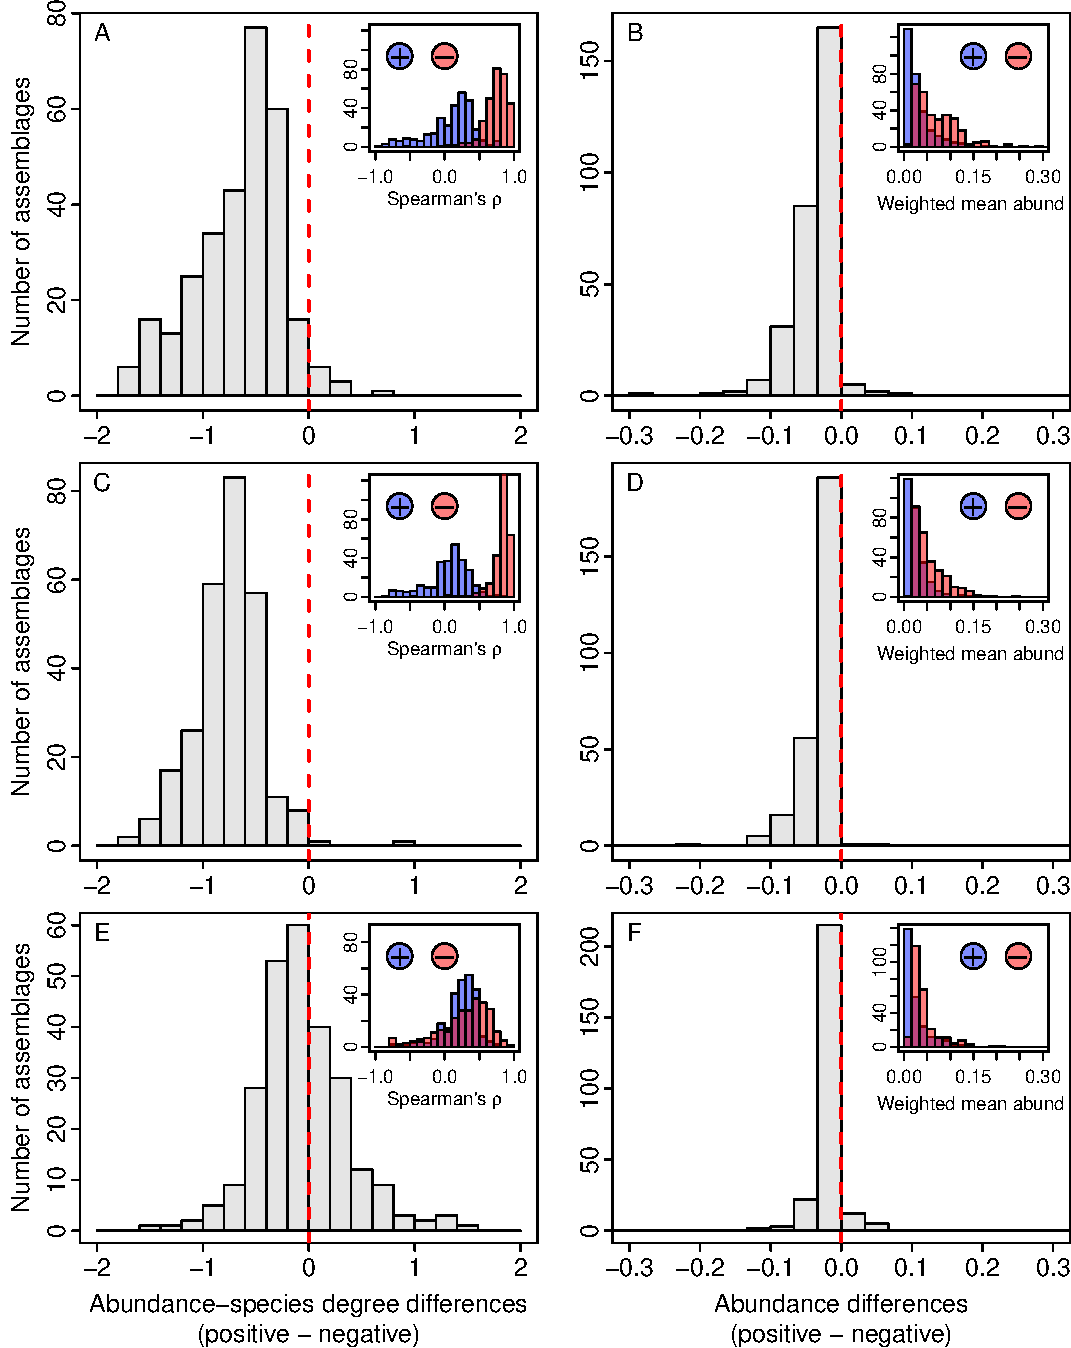
\includegraphics{RarePlusComMinus_files/figure-latex/fig_plusMinus-1} 

}

\caption{Distributions of correlations between network centrality (i.e. species degree) and abundance (left panels) and distributions of weighted mean abundances (right panels). The main figures show the differences between positive and negative association networks, while the inset figures show the sepparate distributions for each network. The results of CEA Figure 2(B-C) are reproduced here in panels A-B; panels C-D show data simulated with a negative binomial SSAD and no species associations; panels E-F show data simulated with a Poisson SSAD and no species associations. \label{fig:plusMinus}}\label{fig:fig_plusMinus}
\end{figure}

In the case of a Poisson SSAD the one parameter (the mean) is fully
specified by the average site-level abundance of a given species. In the
case of a negative binomial SSAD, the mean parameter is again specified
by the site-level average, but the size or clustering parameter \(k\) is
not fully specified. To capture the rough features of the data, I sample
\(k\) from a linear relationship (with noise) between the maximum
likelihood estimates of \(k\) and the relative abundance of each species
(Supplementary Fig. \ref{fig:ssad}).

Figure \ref{fig:plusMinus} A--D shows that with a negative binomial
SSAD, simulated data closely match observed findings: the correlation
between abundance and species' network degree skews more negative in
positive association networks (i.e.~more rare species are more highly
connected in positive association networks), and positive associations
networks tend to contain more rare species than negative networks. This
correspondence between real and simulated patterns largely disappears
when we instead use a Poisson SSAD, highlighting the importance of
spatial aggregation in driving the spurious results.

My findings do not depend on simulating SAD and SSAD shapes from the
data: in Supplementary Figure \ref{fig:simpleSim} I show that the
spurious relationship between abundance and association type occurs even
when simulating data from just one arbitrary SAD function with the one
arbitrary spatially clustered SSAD for all species. In this simulation,
again, replacing the spatially clustered SSAD with a Poisson SSAD breaks
the spurious connection between abundance and association type as in
Figure \ref{fig:plusMinus} (E-F).

Why do negative binomial SSADs reproduce the results while Poisson SSADs
fail to? The null model algorithm used here and in CEA fixes row and
column marginals, thus the empirical shape of the SAD is preserved, and
the \emph{total} abundances (across all species) at each site are also
preserved. However, the way a species' total abundance is allocated
across sites by the null model has a potentially large combinatorial
space to explore. In Figure \ref{fig:ssadPerm} I compare summary
statistics of known SSADs to their permuted counterparts and find that
the null model transforms negative binomial SSADs to a more Poisson
shape, while leaving Poisson SSADs probabilistically unchanged.
Specifically, when starting with a negative binomial SSAD, the null
model inflates the number of sites individuals are allocated to (more
similarly to a Poisson SSAD) and increases the inferred \(k\) parameter,
indicating less spatial clustering in the permuted matrices compared to
their non-permuted, negative binomial starting points.

\begin{figure}

{\centering 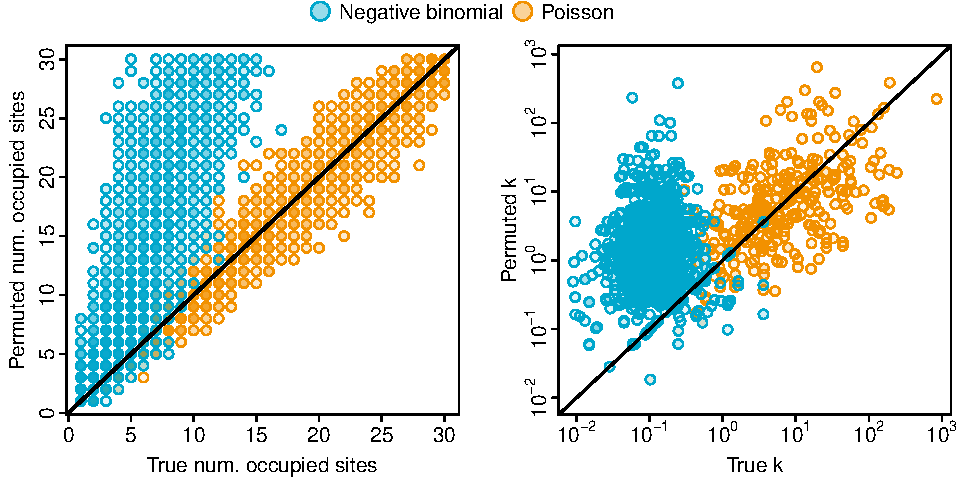
\includegraphics{RarePlusComMinus_files/figure-latex/ssadPerm_plot-1} 

}

\caption{Comparison of SSAD statistics for true and permuted site by species matrices. Colors correspond to the true, un-permuted SSAD. Panel (A) shows how permutation affects number of occupied sites. Panel (B) shows how permutation affects maximum likelihood estimates of the clustering parameter $k$ (B). Points are semi-transparent to help display density. Lines are 1:1 lines. \label{fig:ssadPerm}}\label{fig:ssadPerm_plot}
\end{figure}

The negative binomial SSAD appears to be the key to producing presumably
spurious relationships between abundance and positive or negative
association networks. One might then expect that a null model which
preserves the shape of the SSAD for each species would account for
statistical artifacts deriving from the SSAD. CEA indeed explore such a
null model algorithm (the ``independent swap algorithm'' (Kembel
\emph{et al.}, 2010; Ulrich \& Gotelli, 2010); null model III in the CEA
supplement) and find it still supports their results. I similarly apply
the independent swap algorithm to data simulated with a negative
binomial SSAD and no real species associations or interactions. I find
that the same spurious relationships between abundance and association
type, even when using the independent swap algorithm (Supp. Fig.
\ref{fig:indSwap}). This again confirms that such association networks
and further biological interpretations of them cannot be drawn from
abundance data alone.

At a mathematical level, clustered SSADs as compared to spatially even
SSADs, increase the probability that rare species will appear positively
associated with each other and common species will appear negatively
associated. Consider, for example, two rare species: one with a single
individual and the other with abundance 5, distributed across 5 sites.
Their Schoener similarity is maximized when all individuals occur at the
same site, such as this site by species matrix \[
X_{rare} = \begin{bmatrix} 1 & 5 \\ 0 & 0 \\ 0 & 0 \\ 0 & 0 \\ 0 & 0 \\ \end{bmatrix}
\] If we define \(Q(x_i; \mu = 1)\) as the probability of observing
\(x_i\) individuals in site \(i\) given an SSAD with mean parameter
\(\mu\), then the probability of the above configuration is
\(P(X_{rare}) = Q(5; \mu = 1) \left(Q(0; \mu = 1)^{4}\right)\). Under a
negative binomial SSAD with \(k = 0.1\),
\(P(X_{rare}) = 4.58 \times 10^{-3}\) whereas under a Poisson SSAD
\(P(X_{rare}) = 5.61 \times 10^{-5}\).

Conversely, for two common species, say each with abundance 50, an
example configuration that \emph{minimizes} their Schoener similarity
would be \[
Y_{min} = \begin{bmatrix} 50 & 0 \\ 0 & 50 \\ 0 & 0 \\ 0 & 0 \\ 0 & 0 \\ \end{bmatrix}
\] We calculate the probability of any such scenario where no abundances
overlap as
\(P(Y_{min}) = 4 \left(\left(Q(50; \mu = 10) Q(0; \mu = 10)^{4}\right)^2\right)\).
With a negative binomial SSAD with \(k = 0.1\),
\(P(Y_{min}) = 1.41 \times 10^{-7}\) whereas with a Poisson SSAD
\(P(Y_{min}) = 1.61 \times 10^{-72}\).

We contrast this with a configuration that would \emph{maximize} the
Schoener similarity between these two common species: \[
Y_{max} = \begin{bmatrix} 10 & 10 \\ 10 & 10 \\ 10 & 10 \\ 10 & 10 \\ 10 & 10 \\ \end{bmatrix}
\] The probability of this configuration is
\(P(Y_{max}) = Q(10; \mu = 10)^{10}\). For the same negative binomial
\(P(Y_{max}) = 5.76 \times 10^{-22}\), and for the Poisson
\(P(Y_{max}) = 9.40 \times 10^{-10}\).

Thus a spatially clustered SSAD, compared to a spatially even SSAD,
gives more probability to configurations where rare species appear
aggregated and common species appear over-dispersed. Because the null
model algorithm permutes site by species matrices to resemble more
Poisson-like SSADs this probabilistic difference between spatially
clustered versus even SSADs accounts for the prevalence of rare species
in positive association networks and common species in negative
association networks.

Caution should be used when inferring species association from abundance
data. More fundamentally than the spurious correlation of abundance with
association type, my analysis shows that statistically significant
species associations are inferred from data simulated without any real
species associations. In data simulated with a negative binomial SSAD,
on average 75\% of species were placed in positive association networks
and 75\% in negative association networks with a significance cutoff of
\(\alpha = 0.05\). With the Poisson SSAD these simulated numbers were
72\% for positive networks and 25\% for negative networks. For the
observed data, on average 73\% of species were placed in positive
association networks and 60\% in negative association networks.

It is becoming increasingly appreciated that abundance data alone are
not sufficient to distinguish between different ecological processes
(McGill \emph{et al.}, 2007; Morlon \emph{et al.}, 2009). The question
of why rare species persist is fascinating, and CEA should be commended
for making a concerted effort to illuminate possible mechanisms
underlying the phenomenon; however, to reach robust conclusions, other
types of data, such as actual experimental measurement of shared
environmental associations or species-species interaction strengths, are
needed in addition to abundance data.

\hypertarget{data-and-code-availability}{%
\subsection{Data and Code
Availability}\label{data-and-code-availability}}

All data and code needed to reproduce the results of this manuscript are
available at \url{https://github.com/ajrominger/RarePlusComMinus} and a
detailed description of the analytical approach is available in the
supplement.

\clearpage

\hypertarget{references}{%
\section*{References}\label{references}}
\addcontentsline{toc}{section}{References}

\hypertarget{refs}{}
\begin{CSLReferences}{1}{0}
\leavevmode\hypertarget{ref-barner2018}{}%
Barner, A.K., Coblentz, K.E., Hacker, S.D. \& Menge, B.A. (2018)
Fundamental contradictions among observational and experimental
estimates of non-trophic species interactions. \emph{Ecology},
\textbf{99}, 557--566.

\leavevmode\hypertarget{ref-blanchet2020}{}%
Blanchet, F.G., Cazelles, K. \& Gravel, D. (2020) Co-occurrence is not
evidence of ecological interactions. \emph{Ecology Letters},
\textbf{23}, 1050--1063.

\leavevmode\hypertarget{ref-calatayud2019}{}%
Calatayud, J., Andivia, E., Escudero, A., Melián, C.J., Bernardo-Madrid,
R., Stoffel, M., Aponte, C., Medina, N.G., Molina-Venegas, R., Arnan,
X., Rosvall, M., Neuman, M., Noriega, J.A., Alves-Martins, F., Draper,
I., Luzuriaga, A., Ballesteros-Cánovas, J.A., Morales-Molino, C.,
Ferrandis, P., Herrero, A., Pataro, L., Juen, L., Cea, A. \&
Madrigal-González, J. (2019) Positive associations among rare species
and their persistence in ecological assemblages. \emph{Nat Ecol Evol}.

\leavevmode\hypertarget{ref-carr2019}{}%
Carr, A., Diener, C., Baliga, N.S. \& Gibbons, S.M. (2019) Use and abuse
of correlation analyses in microbial ecology. \emph{The ISME journal},
\textbf{13}, 2647--2655.

\leavevmode\hypertarget{ref-connolly2017}{}%
Connolly, S.R., Hughes, T.P. \& Bellwood, D.R. (2017) A unified model
explains commonness and rarity on coral reefs. \emph{Ecology letters},
\textbf{20}, 477--486.

\leavevmode\hypertarget{ref-engen2008}{}%
Engen, S., Lande, R. \& Sæther, B.-E. (2008) A general model for
analyzing taylor's spatial scaling laws. \emph{Ecology}, \textbf{89},
2612--2622.

\leavevmode\hypertarget{ref-freilich2018}{}%
Freilich, M.A., Wieters, E., Broitman, B.R., Marquet, P.A. \& Navarrete,
S.A. (2018) Species co-occurrence networks: Can they reveal trophic and
non-trophic interactions in ecological communities? \emph{Ecology},
\textbf{99}, 690--699.

\leavevmode\hypertarget{ref-harte2011}{}%
Harte, J. (2011) \emph{The maximum entropy theory of ecology}, Oxford
University Press.

\leavevmode\hypertarget{ref-hubbell2001}{}%
Hubbell, S.P. (2001) \emph{The unified neutral theory of biodiversity
and biogeography}, Princeton University Press.

\leavevmode\hypertarget{ref-hutchinson1961}{}%
Hutchinson, G.E. (1961) The paradox of the plankton. \emph{The American
Naturalist}, \textbf{95}, 137--145.

\leavevmode\hypertarget{ref-picante}{}%
Kembel, S.W., Cowan, P.D., Helmus, M.R., Cornwell, W.K., Morlon, H.,
Ackerly, D.D., Blomberg, S.P. \& Webb, C.O. (2010) Picante: R tools for
integrating phylogenies and ecology. \emph{Bioinformatics}, \textbf{26},
1463--1464.

\leavevmode\hypertarget{ref-kendall1949}{}%
Kendall, D.G. (1949) Stochastic processes and population growth.
\emph{Journal of the Royal Statistical Society. Series B
(Methodological)}, \textbf{11}, 230--282.

\leavevmode\hypertarget{ref-leigh2004}{}%
Leigh Jr, E.G., Davidar, P., Dick, C.W., Terborgh, J., Puyravaud, J.-P.,
Steege, H. ter \& Wright, S.J. (2004) Why do some tropical forests have
so many species of trees? \emph{Biotropica}, \textbf{36}, 447--473.

\leavevmode\hypertarget{ref-mcgill2003}{}%
McGill, B. \& Collins, C. (2003) A unified theory for macroecology based
on spatial patterns of abundance. \emph{Evolutionary Ecology Research},
\textbf{5}, 469--492.

\leavevmode\hypertarget{ref-mcgill2007}{}%
McGill, B.J., Etienne, R.S., Gray, J.S., Alonso, D., Anderson, M.J.,
Benecha, H.K., Dornelas, M., Enquist, B.J., Green, J.L., He, F. \&
others (2007) Species abundance distributions: Moving beyond single
prediction theories to integration within an ecological framework.
\emph{Ecology letters}, \textbf{10}, 995--1015.

\leavevmode\hypertarget{ref-mcgill2005}{}%
McGill, B.J., Hadly, E.A. \& Maurer, B.A. (2005) Community inertia of
quaternary small mammal assemblages in north america. \emph{Proceedings
of the National Academy of Sciences}, \textbf{102}, 16701--16706.

\leavevmode\hypertarget{ref-morlon2009}{}%
Morlon, H., White, E.P., Etienne, R.S., Green, J.L., Ostling, A.,
Alonso, D., Enquist, B.J., He, F., Hurlbert, A., Magurran, A.E. \&
others (2009) Taking species abundance distributions beyond individuals.
\emph{Ecology Letters}, \textbf{12}, 488--501.

\leavevmode\hypertarget{ref-rcore}{}%
R Core Team (2018) \emph{R: A language and environment for statistical
computing}, R Foundation for Statistical Computing, Vienna, Austria.

\leavevmode\hypertarget{ref-rajala2019}{}%
Rajala, T., Olhede, S.C. \& Murrell, D.J. (2019) When do we have the
power to detect biological interactions in spatial point patterns?
\emph{Journal of Ecology}, \textbf{107}, 711--721.

\leavevmode\hypertarget{ref-sander2017}{}%
Sander, E.L., Wootton, J.T. \& Allesina, S. (2017) Ecological network
inference from long-term presence-absence data. \emph{Scientific
reports}, \textbf{7}, 7154.

\leavevmode\hypertarget{ref-schoener1968}{}%
Schoener, T.W. (1968) The anolis lizards of bimini: Resource
partitioning in a complex fauna. \emph{Ecology}, \textbf{49}, 704--726.

\leavevmode\hypertarget{ref-ulrich2010}{}%
Ulrich, W. \& Gotelli, N.J. (2010) Null model analysis of species
associations using abundance data. \emph{Ecology}, \textbf{91},
3384--3397.

\leavevmode\hypertarget{ref-yenni2012}{}%
Yenni, G., Adler, P.B. \& Ernest, S.M. (2012) Strong self-limitation
promotes the persistence of rare species. \emph{Ecology}, \textbf{93},
456--461.

\leavevmode\hypertarget{ref-zillio2010}{}%
Zillio, T. \& He, F. (2010) Modeling spatial aggregation of finite
populations. \emph{Ecology}, \textbf{91}, 3698--3706.

\end{CSLReferences}

\end{document}
